\graphicspath{{./}{./figures/}{./figures/torchsynth/}}

\chapter{GPU Enabled Synthesis}

\section{Introduction}
\label{sec:intro}

Machine learning progress has been driven by training regimes that leverage large corpora. The past decade has seen great progress in NLP and vision tasks using large-scale training. As early as 2007, Google \cite{brants-etal-2007-large} achieved state-of-the-art machine translation results using simple trillion-token $n$-gram language models.
Recent work like GPT3 \cite{NEURIPS2020_1457c0d6} suggests that it is preferable to do less than one epoch of training on a large corpus, rather than multiple epochs over the same examples. Even tasks with little training data can be attacked using self-supervised training on a larger, related corpus followed by a transfer-learning task-specific fine-tuning step.

\begin{table}[thb]
\begin{center}
\begin{tabular}{r|c|r|c|c}
Name & Type & \#hours & Free & Multi-modal \\
\hline
Diva \cite{esling2020flow} & synth & 12 & yes & parameters \\
FSDK50 \cite{fonseca2020fsd50k} & broad & 108 & yes & tags \\
NSynth \cite{engel2017neural} & notes & 333 & yes & tags \\
LibriSpeech \cite{librispeech} & speech & 1000 & yes & text \\ 
DAMP-VPB \cite{smule_inc_2017_2616690} & songs & 1796 & no & lyrics \\
Audioset \cite{45857} & broad & 4971 & no & video+tags \\ 
YFCC100M \cite{thomee2016yfcc100m} & broad & 8081 & yes & video \\
MSD \cite{bertin2011million} & songs & 72222 & no & tags+metadata \\
Jukebox \cite{dhariwal2020jukebox} & songs & 86667 & no & {\footnotesize lyrics+metadata}\\
synth1B1 & synth & 1111111 & yes & parameters \\
% etc let's add a few more standard corpora here
% also the SMULE zenodo singing corpus
\end{tabular}
\end{center}
\caption{Large-scale and/or synthesizer audio corpora.}
\label{tbl:audio-corpora}
\end{table}

Unfortunately, audio ML progress has been hindered by a dearth of large-scale corpora. Audio ML involves multiple epoch training on comparably small corpora compared to vision or NLP. Table~\ref{tbl:audio-corpora} summarizes various large-scale and/or synthesizer audio corpora.
For example, using AudioSet \cite{45857} requires scraping 5000 hours of Youtube videos, many of which become unavailable over time (thus impeding experimental control). FSD50K \cite{fonseca2020fsd50k}, a free corpus, was recently released to mitigate these issues, but contains only 108 hours of audio. To the best knowledge of the authors, the largest audio set used in published research is Jukebox \cite{dhariwal2020jukebox}, which scraped 1.2M songs and their corresponding lyrics. Assuming average song length is 4:20, we estimate their corpus is $\approx$90K hours. 



\subsection{Background and Motivation}

\subsubsection{Pre-training and learned representations}

Tobin {\em et al.}~\cite{DBLP:conf/iros/TobinFRSZA17} argue that learning over synthesized data enables transfer learning to the real-world.
Multi-modal training offers additional benefits.
Images evince sizes of objects immediately, while object size is difficult to glean through pure linguistic analysis of large corpora  \cite{DBLP:conf/acl/ElazarMRBR19}.
Multi-model learning of audio---with video in \cite{DBLP:conf/icassp/CramerWSB19} and semantic tags in \cite{drossos:icml:2020}---has led to strong audio representations.
Constrastive audio learning approaches like \cite{saeed2020contrastive} can be used in multi-modal settings, for example by learning the correspondence between a synthesized sound and its underlying parameters.
% Later, cite BYOL-A if their paper is selected
However, training such models is limited by small corpora and/or the relatively slow synthesis speed of traditional CPU-based synths (Niizumi, p.c.).

\subsubsection{Software Synthesizers}

Programming audio synthesizers is challenging and requires a technical understanding of sound design to fully realize their expressive power. Traditional synthesizers can have over 100 parameters that affect audio generation in complex, non-linear ways. One of the most commercially successful audio synthesizers, the Yamaha DX7, was notoriously challenging to program. Allegedly nine out of ten DX7s coming into workshops for servicing still had their factory presets intact \cite{seago2004critical}.

Since the early 90s, researchers have leveraged advances in ML to develop a deeper understanding of the synthesizer parameter space and to build more intuitive methods for interaction \cite{horner1993machine}. Recently, deep learning has been used for programming synthesizers.  Esling {\em et al.}\ \cite{esling2020flow} trained an auto-encoder network to program the \href{https://u-he.com/products/diva/}{U-He Diva} using 11K synthesized sounds with known preset values. Yee-King {\em et al.} \cite{yee2018automatic} used a recurrent network to automatically find parameters for \href{https://asb2m10.github.io/dexed/}{Dexed}, an open-source software emulation of the DX7.

\subsubsection{Neural Synthesis}

In contrast to traditional synthesis, neural synthesizers generate audio using large-scale machine learning architectures with millions of parameters \cite{engel2017neural}. Differentiable digital signal processing \cite{engel2020ddsp} bridged the gap between traditional DSP synthesizers with the expressiveness of neural networks, exploring a harmonic model-based approach, using a more compact architecture with 100K parameters.
One benefit of synthesized audio is that the underlying factors of variation ({\em i.e.}~the parameters) are known. We combine the ideas of traditional DSP and neural synthesis, yielding a greater level of simplicity and speed by building a GPU-optional modular synthesizer. Our default voice has 78 latent parameters, which model traditional synthesizer parameters. 

\section{Main Contributions}
\label{sec:contributions}

Our synth1B1 corpus and torchsynth software provide a fast, open approach for researchers to do large-scale audio ML pre-training and develop a deeper understanding of the complex relationship between the synthesizer parameter space and resulting audio.
A variety of existing research problems can use synth1B1, including:
\begin{itemize}
\item Perceptual research into audio, such as crafting auditory distance measures and inferring timbre dimensions. \cite{vahidi2020timbre}
\item Inverse synthesis, i.e.\ mapping from audio to underlying synthesis parameters.
\cite{yee2018automatic,esling2020flow}
\item Inferring macro-parameters of synthesizers that are more perceptually relevant. \cite{esling2020flow, tatar2020latent}
%\item Transfer learning for automatic programming of black-box software synthesizers.
\item Audio-to-MIDI. \cite{47659}
\item Imitation of natural sounds with established synthesis architectures.
\end{itemize}
%% can you think of more?
Researchers can also use the synth1B1 corpus to arbitrage innovations from adjacent ML fields, namely: large-scale multi-modal, self-supervised, and/or contrastive learning, and transfer-learning through fine-tuning on the downstream task of interest, particularly tasks with few labeled examples.

\subsection{synth1B1}

synth1B1 is a corpus consisting of one million hours of audio: one billion 4-second synthesized sounds. The corpus is multi-modal: Each sound includes its corresponding synthesis parameters. We use deterministic random number generation to ensure replicability, even of noise oscillators. One tenth of the examples are designated as the test set. Researchers can denote subsamples of this corpus as synth1M1, synth10M1, {\em etc.} % which would refer to the first 1 million and 10 million samples of Synth1B1 respectively.

Data augmentation has been used on small-scale corpora to increase the amount of labeled training data. As discussed in \S\ref{sec:intro}, large-scale one-epoch training is preferable, which is possible using synth1B1's million-audio-hours.

Besides sheer size, another benefit of synth1B1 is that it is multi-modal: instances consist of both audio {\em and} the underlying parameters used to generate this audio. The use of traditional synthesis paradigms allows researchers to explore the complex interaction between synthesizer parameter settings and the resulting audio in a thorough and comprehensive way. 
Large-scale contrastive learning typically requires data augmentation ({\em e.g.}\ image or spectrogram deformations) to construct positive contrastive-pairs \cite{pmlr-v119-chen20j,DBLP:journals/corr/abs-2103-06695}. However, this sort of faux-constrastive-pair creation is not necessary when the underlying latent parameters are known in a corresponding modality.

\subsection{torchsynth}

synth1B1 is generated {\em on the fly} by \href{https://github.com/torchsynth/torchsynth}{torchsynth 1.0}.
% TODO: pypi package
% TODO: We could make a 'torchsynth' github org rather than using my namespace
torchsynth is an open-source modular synthesizer and is GPU-enabled. torchsynth renders audio at 16200x real-time on a single V100 GPU. Audio rendered on the GPU can be used in downstream GPU learning tasks without the need for expensive CPU-to-GPU move operations, not to mention disk reads. It is faster to render synth1B1 {\em in-situ} than to download it. torchsynth includes a replicable script for generating synth1B1.
 %Many modules in torchsynth 1.0 are differentiable but backprop has not been stress-tested in this release, as our focus has been fast inference and perceptual sonic diversity. % [also the discussion on those guys that did their own differentiation things from FB chat]
To accommodate researchers with smaller GPUs, the default batchsize is 128, which requires between 1.9 and 2.4 GB of GPU memory, depending upon the GPU.
%The nomenclature ``synth1B1-312-6'' denotes batch 312 and sound 6 within that batch.
If a train/test split is desired, 10\% of the samples are marked as test. Because researchers with larger GPUs seek higher-throughput with batchsize 1024, $9 \cdot 1024$ samples are designated as train, the next 1024 samples as test, {\em etc.} The default sampling rate is 44.1kHz. However, sounds can be rendered at any desired sample rate. %, such as 96kHz, for use in high-resolution applications.
% What about fp16?
Detailed instructions are contained at the torchsynth URL for the precise protocol for replicably generating synth1B1 and sub-samples thereof. %(See profiling in Section [...]).

% We might also need to be careful because if we exhaust the space of possible sounds of the synthesizer, then a simple KNN approach will find the right parameters.

%JND experiments demonstrates that [...]\% of audio samples are perceptually different to human listeners.
%[multimodal]

\subsection{Questions in Synthesizer Design, and New Pitch and Timbre Datasets and Benchmarks}

When generating synthesized datasets, one needs to sample the parameter space. Typically this is achieved through na\"ively sampling parameters uniformly and rendering the resulting audio. Due to the complexity of the parameter space and interaction between parameters, this may lead to a large number of redundant, extreme frequency, and/or unnatural sounds. We propose several new open challenges in synthesizer design, specifically focusing on the task of designing parameters and sampling them, including:
\begin{itemize}
    \item How do you measure the perceptual diversity of a synthesizer's sounds? How do you maximize it?
    \item How do you tune a synthesizer to imitate existing synthesizers? Is there a way to sample the parameters so the resulting audio sounds like a human-designed preset?
\end{itemize}
In \S\ref{sec:hyperparameter-tuning} we demonstrate a principled approach to attacking these tasks. The main research barrier to solving these tasks is the lack of an automatic, perceptually-relevant auditory distance measures.
To evaluate existing auditory distance measures, we devise two new evaluation methodologies and concurrently release timbre and pitch-datasets, each representing 22.5 and 3.4 hours of audio respectively, for the following open-source synthesizers: a \href{https://github.com/bwhitman/learnfm}{DX7} clone and \href{https://surge-synthesizer.github.io/}{Surge}, as \href{https://zenodo.org/record/4677102}{DOI 10/f7dg} and \href{https://zenodo.org/record/4677097}{DOI 10/f652}, respectively. These datasets represent ``natural'' synthesis sounds---i.e.\ presets designed by humans, not just a computer randomly flipping knobs---which we use in two ways: a) New benchmarks for evaluating audio representations. b) Evaluating the similarity of different sound corpora.
%[Secret Sauce data if they grant us license] Lastly, we release a standardized format for describing the parameter settings and appropriate ranges and scaling.


\section{Design Methodology}
\label{sec:design-methodology}
\subsection{Synth Modules}
torchsynth's design is inspired by hardware modular synthesizers which contain individual units. Each module has a specific function and parameters, and they can be connected together in various configurations to construct a synthesizer. There are three types of modules in torchsynth: audio modules, control modules, and parameter modules. Audio modules operate at audio sampling rate (default 44.1kHz) and output audio signals. Examples include voltage-controlled oscillators (VCOs) and voltage-controlled amplifiers (VCAs). Control modules output control signals that modulate the parameters of another module. For speed, these modules operate at a reduced control rate (default 441Hz). Examples of control modules include ADSR envelope generators and low frequency oscillators (LFOs). Parameter modules simply output parameters. An example is the monophonic ``keyboard'' module that has no input, and outputs the note midi f0 value and duration.

To take advantage of the parallel processing power of a GPU, all modules render audio in batches. Larger batches enable higher throughput on GPUs.  Figure~\ref{fig:gpu-profiles} shows torchsynth's throughput at various batch sizes on a single GPU. GPU memory consumption $\approxeq 1216 + (8.19\ \cdot $ batch\_size) MB, including the torchsynth model. The default batch size 128 requires $\approx$2.3GB of GPU memory, and is 16200x faster than realtime on a single V100 GPU. %Any multiple of 128 batch-size is supported and synth1B1 will be deterministically rendered for scientific reproducibility.
A batch of 4 of randomly generated ADSR envelopes is shown in Figure~\ref{fig:adsr}.


%\renewcommand{\thesubfigure}{Figure %\arabic{subfigure}}

\begin{figure}[t]
    \centering
    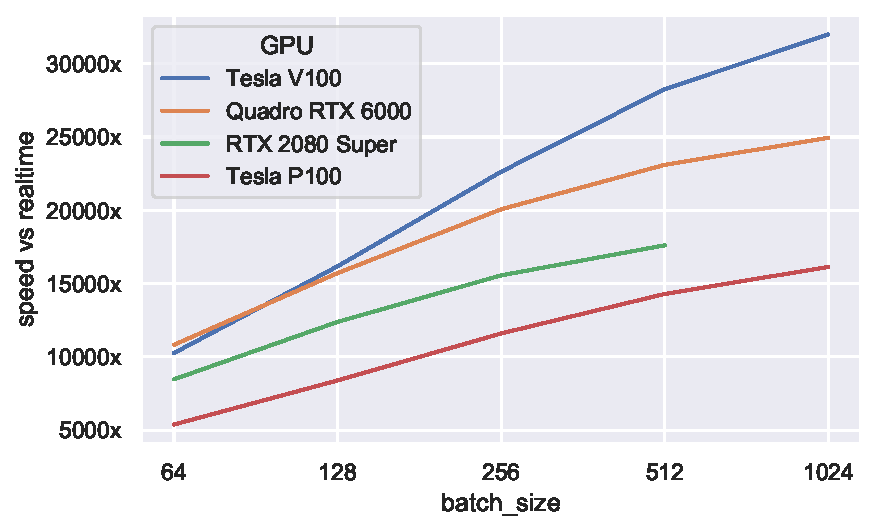
\includegraphics[width=0.66\linewidth]{gpu-profiles.pdf}
  \vspace{-1.5em}
    \caption{torchsynth throughput at various batch sizes.}
    \label{fig:gpu-profiles}
\end{figure}

\begin{figure}[t]
    \centering
    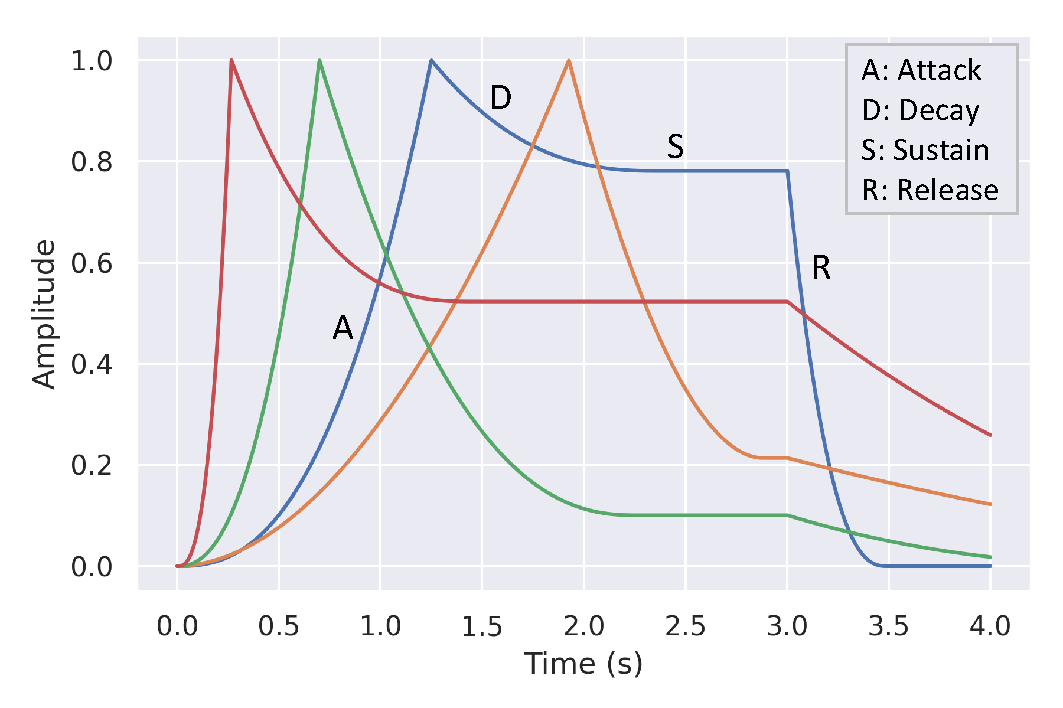
\includegraphics[width=0.66\linewidth]{ADSR.pdf}
%    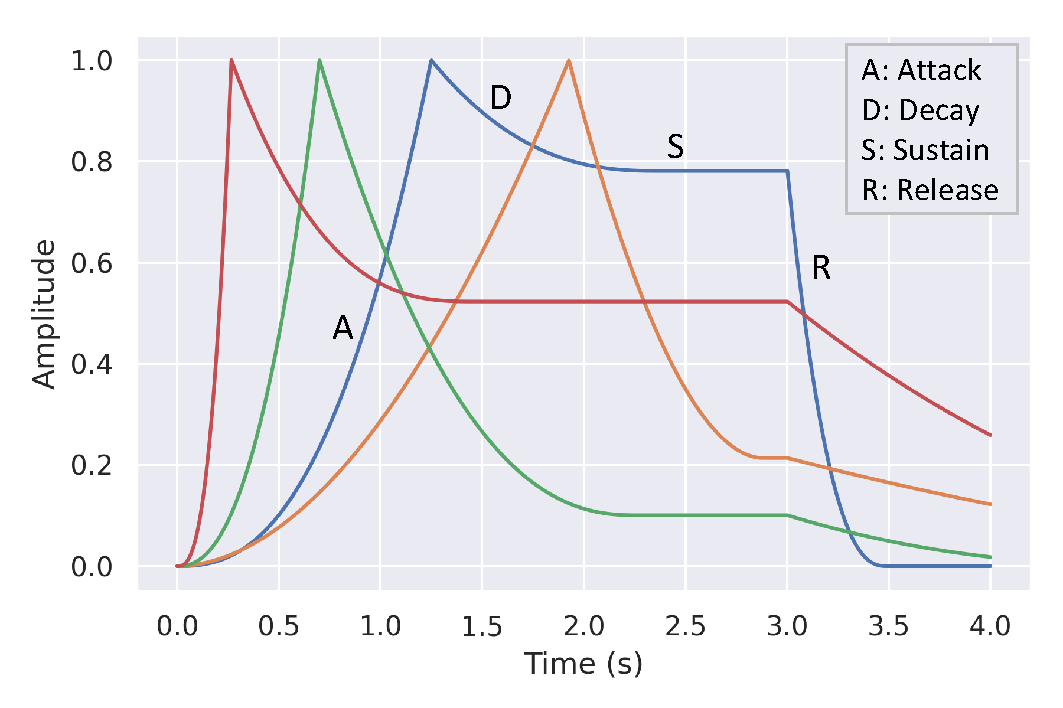
\includegraphics[width=0.95\linewidth]{ADSR.pdf}
  \vspace{-1.5em}
    \caption{Batch of four randomly generated ADSR envelopes.
    Each section for one of the envelopes is labelled.}
    \label{fig:adsr}
\end{figure}

\subsection{Synth Architectures}

The default configuration in torchsynth is the Voice, which is the architecture used in synth1B1. The Voice comprises the following modules: a Monophonic Keyboard, two LFOs, six ADSR envelopes (each LFO module includes two dedicated ADSRs: one for rate modulation and another for amplitude modulation), one Sine VCO, one SquareSaw VCO, one Noise generator, VCAs, a Modulation Mixer and an Audio Mixer. Modulation signals generated from control modules (ADSR and LFO) are upsampled to the audio sample rate before being passed to audio rate modules. Figure \ref{fig:voice_diagram} shows the configuration and routing of the modules comprised by Voice. 

\begin{figure}[t]
    \centering
    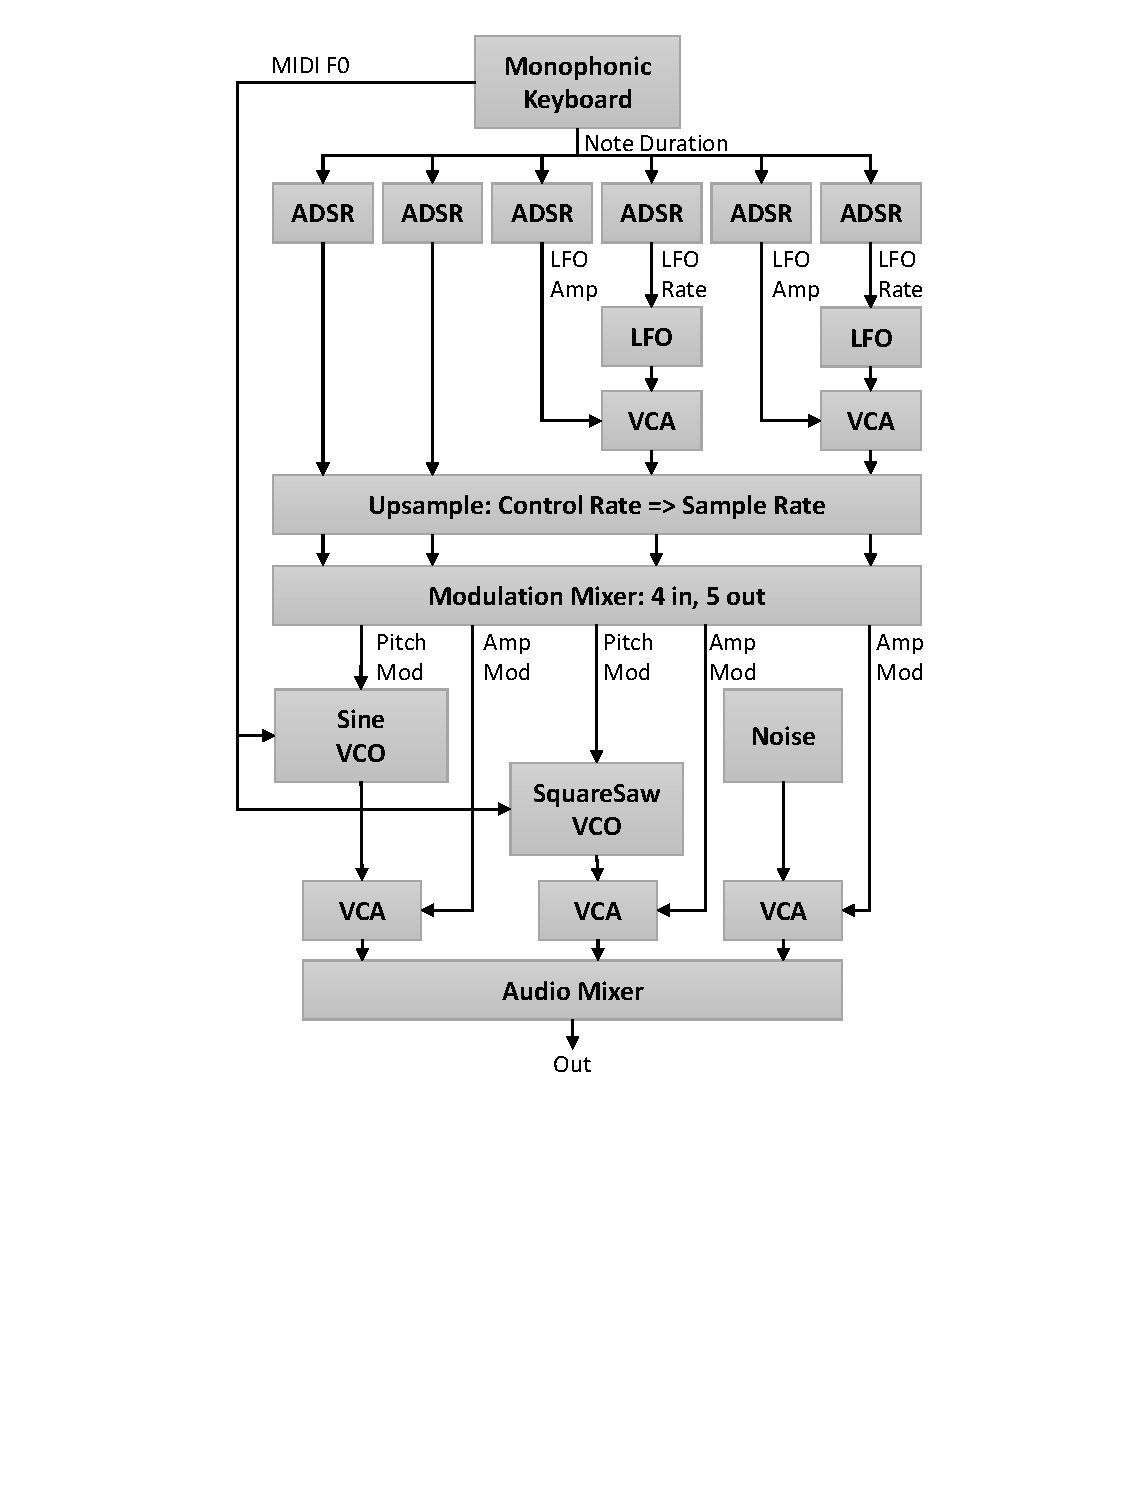
\includegraphics[width=0.5\linewidth]{SynthDiagram_3.pdf}
  \vspace{-1.5em}
    \caption{Module configuration for the Voice in torchsynth}
    \label{fig:voice_diagram}
\end{figure}

%The Voice module is strictly additive and contains no filter.
%Our principle design imperative was fast throughput using traditional synthesis modules, followed by expressivity. Designing fast expressive GPU-enabled filters is an open research question. Infinite Impulse Response (IIR) filters are expressive but require recursive computation, thus impeding computation speed on a GPU \cite{iir}. Kuznetsov {\em et al.}\ \cite{iir} argue that convolution neural networks can be viewed as non-linear Finite Impulse Response (FIR) filters and the promising results of differentiable FIRs used in Engel {\em et al.}\ \cite{engel2020ddsp}
% and Bitton {\em et al.}\ 
%\cite{DBLP:journals/corr/abs-2008-01393} suggest directions for future work. 
While the Voice is the default architecture of torchsynth 1.0, any number of synth architectures can be configured using the available modules. For example, a 4-operator frequency modulation (FM) \cite{chowning1973synthesis} synthesizer inspired by \href{https://www.ableton.com/en/packs/operator/}{Ableton Live's Operator instrument} is currently in development.

\begin{figure}[thb]
    \centering
    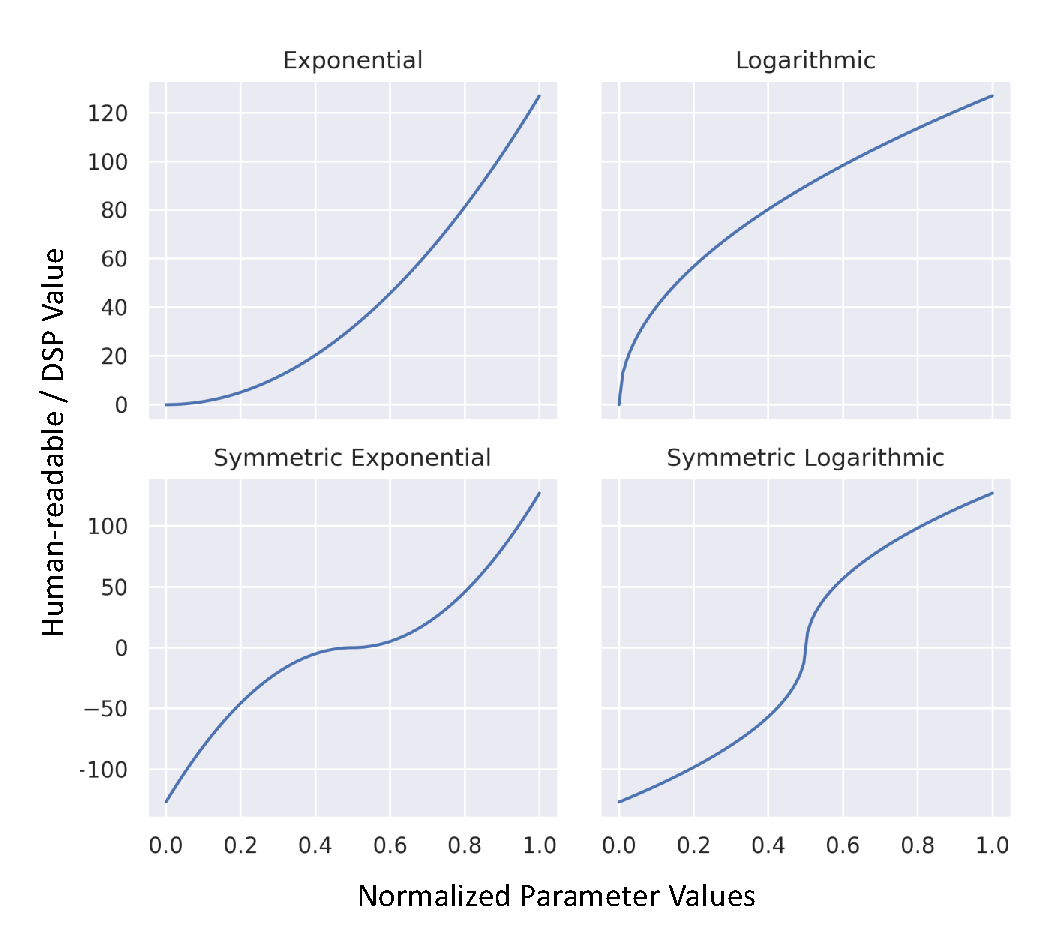
\includegraphics[width=0.95\linewidth]{Hyperparam_4.pdf}
    \caption{Examples of parameter curves used to convert to and from normalized parameter values and the human-readable values used in the DSP algorithms. The top two curves are non-symmetric curves, mapping to values in the range [0, 127]. The bottom two curves are symmetric, mapping to values in the range [-127, 127].}
    \label{fig:parameter_curves}
\end{figure}

\subsection{Parameters}
Module parameters can be expressed in human-readable form with predetermined min and max values, such as $0 \le \textrm{midi f0} \le 127$. These human-intepretable values are used by the DSP algorithms of each module.
Internally, parameters are stored in a corresponding normalized range $[0, 1]$. synth1B1 parameters are sampled uniformly from the normalized range. However, there is potentially a non-linear mapping between the internal range and the human-readable range. Besides the fixed min and max human-readable values, each parameter has hyperparameters ``curve'' and ``symmetry'' that determine how internal [0, 1] values are transformed to the human-readable values. The curve can specify a particular logarithmic, linear, or exponential sampling approach, {\em e.g.}\ to emphasize higher or lower values. Symmetric curves, which alternately emphasize the center or edges of the distribution, are used for parameters such as oscillator tuning where the default value is 0 and can take on a range of both positive and negative values. An example set of non-linear curves is shown in Figure \ref{fig:parameter_curves}.

In our nomenclature, a particular choice of hyperparameter settings, which correspond to random sample space of markedly different sonic character, are called {\em nebulae}. The initial Voice nebula was designed by the authors based upon intuition and prior experience with synthesizers. We experiment with tuning the hyperparameters of Voice to generate different nebulae in \S\ref{sec:hyperparameter-tuning}.

%\subsection{Perceptual motivation for initial hyperparameter choices}

%[ddsp]

%[blah blah blah some of the modules we have implemented]

% [How did we pick the boundaries and scaling]

%[How did we motivate it perceptually]


%\section{Profiling}

%[profile on various GPUs]

%[realtime not throughput]

%[other synths]

%[neural granular synth]

%[speed profiles vs various synths, including wavenets, renderman, surge python, DDSP]

\section{Evaluation of Auditory Distances}

We seek to quantify the diversity of sounds that can be generated with torchsynth, given a particular nebula; or similarly, to quantify to what extent a certain nebula can capture the variability of sounds in another dataset. In order to do so, we first need a reliable measure of similarity or dissimilarity between pairs of sounds, also known as an auditory distance. 

Auditory distances have many applications in audio ML. They provide the basis for quantitative evaluation and optimization criteria. In a sense, the auditory distance measure is the ``ear'' of a model. For example, auditory distances can be used to evaluate the similarity of two sounds that were generated by different synthesis engines. By extension, a well-tuned distance could estimate whether two sounds are perceptually indistinguishable to human listeners. For example, a 4-second sinusoid at 30~kHz, when compared to 4-seconds of silence, should have an auditory distance of zero if the distance is properly tuned to the typical range of human hearing. Likewise, two random instances of white noise should have a perceptual distance of zero, or near zero, despite their entirely different waveforms.

Auditory distances typically involve computing some multidimensional representation of a sound, then computing a distance over the representation space \cite{turian2020im}.
To perform a controlled evaluation of auditory distances, we devised two experiments using two new datasets.
Sounds in each dataset are RMS-level normalized using the \href{https://github.com/kklobe/normalize}{normalize} package.


\begin{table}[ht]
  \centering
  \begin{tabular}{rlcrrrrrr}
{} & & & \multicolumn{3}{c}{Spearman with a preset} & \multicolumn{3}{c}{DCG across presets} \\
 &  &  &  & Surge & DX7 &  & Surge & DX7 \\
Representation & model choice & normed &  & pitch & velocity & mean & &  \\
\hline
OpenL3 \cite{Cramer:LearnMore:ICASSP:19} & env, mel256, 6144  &              &          \textbf{0.821} &           \textbf{0.746} &              0.896 &             0.880 &              0.908 &                 0.852 \\
OpenL3 \cite{Cramer:LearnMore:ICASSP:19}& env, mel256, 6144 & \checkmark     &          \textbf{0.821} &           \textbf{0.747} &              0.895 &             0.809 &              0.883 &                 0.735 \\
OpenL3 \cite{Cramer:LearnMore:ICASSP:19} & music, mel256, 6144 & \checkmark   &          0.817 &           0.732 &              \textbf{0.903} &             0.820 &              0.916 &                 0.724 \\
OpenL3 \cite{Cramer:LearnMore:ICASSP:19} & music, mel256, 6144  &            &          0.813 &           0.722 &              \textbf{0.903} &             0.892 &              \textbf{0.942} &                 0.842 \\
Coala \cite{drossos:icml:2020} & dual\_ae\_c & \checkmark                    &          0.813 &           0.729 &
 0.896 &             0.555 &              0.547 &                 0.564 \\
Coala \cite{drossos:icml:2020} & dual\_e\_c & \checkmark                     &          0.811 &           0.737 &
 0.884 &             0.569 &              0.576 &                 0.563 \\
 
NSynth Wavenet \cite{engel2017neural} & & \checkmark                            &          0.810 &           0.717 &              \textbf{0.903} &             0.582 &              0.591 &                 0.573 \\
OpenL3 \cite{Cramer:LearnMore:ICASSP:19} & music, linear, 6144 &             &          0.808 &           0.722 &              0.895 &             0.874 &              \textbf{0.943} &                 0.805 \\
OpenL3 \cite{Cramer:LearnMore:ICASSP:19} & music, mel256, 512 &              &          0.804 &           0.710 &              0.899 &             \textbf{0.904} &              \textbf{0.943} &                 \textbf{0.864} \\
OpenL3 \cite{Cramer:LearnMore:ICASSP:19} & music, mel256, 512 & \checkmark    &          0.801 &           0.705 &              0.897 &             0.585 &              0.606 &                 0.564 \\
NSynth Wavenet \cite{engel2017neural} & &                                     &          0.789 &           0.675 &              \textbf{0.903} &             0.835 &              0.893 &                 0.777 \\
Coala \cite{drossos:icml:2020} & dual\_ae\_c &                              &          0.776 &           0.658 &              0.893 &             0.748 &              0.756 &                 0.740 \\
Coala \cite{drossos:icml:2020} & dual\_e\_c &                               &          0.750 &           0.630 &
 0.871 &             0.681 &              0.710 &                 0.652 \\
Multi-scale spectrogram \cite{engel2020ddsp,steinmetz2020auraloss} & linear+log, [4096 ... 64] & &          0.792 &           0.690 &              0.894 &             0.543 &              0.555 &                 0.531 \\
Multi-scale spectrogram \cite{engel2020ddsp,steinmetz2020auraloss} & log, [4096 ... 64] & &          0.786 &           0.689 &              0.884 &             0.542 &              0.566 &                 0.518 \\
Multi-scale spectrogram \cite{engel2020ddsp,steinmetz2020auraloss} & linear, [4096 ... 64] & &          0.658 &           0.410 &              \textbf{0.905} &             0.447 &              0.343 &                 0.551 \\
Coala \cite{drossos:icml:2020} & cnn & \checkmark                          &          0.555 &           0.303 &              0.806 &             0.485 &              0.433 &                 0.537 \\
Coala \cite{drossos:icml:2020} & cnn &                                   &          0.552 &           0.297 &              0.807 &             0.714 &              0.614 &                 0.815 \\
 \end{tabular}
  \caption{Performance of representations on experiments defined in \S~\ref{sec:experiment1} and \ref{sec:experiment2}. Best scores, and scores within 0.002 of the best, are bold-faced. $\ell_1$ distance was used because it outperformed $\ell_2$. We sort by mean spearman within a preset.
  }
  \label{tab:distance-eval}
\end{table}


\subsection{DX7 Timbre Dataset}
\label{sec:dx7}

Given 31K unique human-devised presets for the DX7\footnote{We used this clone: \url{github.com/bwhitman/learnfm}}, we generated 4-second samples on a fixed midi pitch (69 = A440) with a note-on duration of 3 seconds. For each preset, we varied only the velocity, from 1--127. This dataset is built on the hypothesis---verified through informal listening tests---that velocity, while carrying no timbral information itself, effects a meaningful, monotonic variation in timbre when it is explicitly programmed into a DX7 patch. Not all DX7 patches are velocity sensitive, and some are more sensitive than others. Sounds that were completely identical---{\em i.e.} each sample matched with error 0---were removed from the dataset. 8K presets had only one unique sound. The median was 51 unique sound per preset, mean 41.9, stddev 27.4.

\subsection{Surge Pitch Dataset}
\label{sec:surge}

The open-source \href{https://surge-synthesizer.github.io/}{Surge synthesizer} is a versatile subtractive synthesizer with a variety of oscillator algorithms: Classic, Sine, Wave-table, Window, FM2, FM3, S\&H Noise and Audio Input. To explore another dimension of variability, in this case {\em pitch}, we used the \href{https://github.com/surge-synthesizer/surge-python}{Surge synthesizer Python API} and the 2.1K standard Surge presets. Here we held the velocity constant at 64, and varied midi pitch values from 21--108, the range of a grand piano. Only a small percentage of presets (like drums and sound effects) had no meaningful pitch variation, and thus no perceptual ordering as pitch increases. However, the inclusion of noise in many of these sounds precluded the use of automatic filtering of perceptually indistinct sounds. Therefore, a small fraction of presets are unclassifiable, imposing a uniform upper bound in accuracy across the board for all auditory distances.
%This small set perceptually unclassifiable was controlled for in our experiments by applying all distances to the exact same presets and sounds, {\em i.e.}\ the small percent of perceptually unrankable presets penalized all distances equally.

\subsection{Distance Experiment 1: Timbral and Pitch Ordering Within a Preset}
\label{sec:experiment1}

In this experiment, we measure the ability of an auditory distance to order sounds by timbre, or by pitch, in the DX7 and Surge datasets, respectively. In effect, the experiment is two evaluations in parallel, run on two separate datasets.

We sample a random preset with at least 3 unique sounds. For each sound $s$, we pick a random sound $s_l$ from this preset with a lower rank (using the DX7 set, this would be a sound having the same pitch but a lower velocity; for the Surge dataset this is a sound having the same velocity but lower pitch); and a random sound $s_h$ with higher rank. %We do not use the min and max rank sounds because they sometimes have unusual timbres, and also to improve experimental control overall. 

For each of $s$, $s_l$ and $s_h$, we compute the distance $d(\cdot, \hat{s})$ between this sound and all other sounds $\hat{s}$ in the dataset. While $s$ is the sample of interest, distance measures are strictly non-negative. Therefore, we seek a concurrent metric to determine whether the compared sound $\hat{s}$ is ``above'' or ``below'' $s$. If the sound $\hat{s}$ is closer to $s_l$, we determine the sign of the distance to $s$ to be negative. If $\hat{s}$ is closer to $s_h$, we determine the sign of the distance to $s$ be positive. As a result, we have a signed distance metric comparing the sound $s$ to every other sound in the dataset.

This set of distances is then correlated to the ground-truth index of pitch, or velocity (depending on the dataset). The correlation, here a Spearman rank correlation, reflects the extent to which the signed distance can properly order the dataset by variability in pitch or velocity. 
One limitation of this methodology for inducing a forced ranking from simple distance is that if, say, $s = 80, s_l = 31, s_h = 81,$ and $\hat{s} = 79$, we might judge $\hat{s}$ as closer to $s_h$ and thus above $s$. We controlled for this by using the same choice for every auditory distance of $s_h$ and $s_l$ given $s$.

Formally, we estimate:
\begin{align}
\begin{split}
\mathop{\mathbb{E}}_{S \in P, s \in S, s_l, s_h \sim S, s_l < s < s_h} \bigg [ \mathop{\rho}_{\hat{s} \in S}\Big (& \textrm{rank}(\hat{s}), d(s, \hat{s}) \ \cdot \\
& \textrm{sgn} \big (d(s_h, \hat{s}) < d(s_l, \hat{s} \big ) \Big) \bigg ]
\end{split}
\end{align}
$P$ is the set of presets, $S$ sounds in that preset, and $\rho$ is spearman.

% Turian adds interstitial magic...

%If $d(s_l, \hat{s}) < d(s_h, \hat{s})$, we negate the distance $-d(s, \hat{s})$ because we assume it is lower rank. Given all distances $d(s, \hat{s})$---some of which are possibly negated---we compute the spearman correlation of the predicted ranks against the true ranks of the sounds within this preset. Spearmans are micro-averaged, i.e., correlations are weighted by the size of constituent presets, over 150 presets, so presets with few timbres are not over-represented.






\subsection{Distance Experiment 2: Determine a Sound's Preset}
\label{sec:experiment2}

A good distance measure should have low distance between sounds generated by the same preset. For each trial, we sample 200 different presets. We sample 2 unique sounds from each preset. For each sound, we compute its distance against the 399 other sounds, and then compute the discounted cumulative gain (DCG) \cite{pmlr-v30-Wang13} of the sound from the same preset, with binary relevance. The DCG is computed for all 400 sounds in the trial. We perform 600 trials.

In the Surge dataset, to control for the helical nature of pitch perception \cite{shepard1982geometrical}, the second sound was always an interval of six semitones (AKA a tritone, {\em diabolus in musica}) from the first note. This ensured that pitches were close, but avoided similar partials due to overlapping harmonics that could be easily matched.

\subsection{Evaluation Results}

To evaluate the perceptual similarity between two audio samples, we need a good representation to compute distances: a) The multi-scale spectrogram distance has been used in a variety of applications, particularly in speech synthesis \cite{wang_neural_2019,DBLP:conf/icassp/YamamotoSK20} but also in music \cite{DBLP:journals/corr/abs-2008-01393,engel2020ddsp,dhariwal2020jukebox};
b) NSynth Wavenet \cite{engel2017neural} is a Wavenet-architecture trained on NSynth musical notes; c) OpenL3 \cite{Cramer:LearnMore:ICASSP:19} was  trained multi-modally on AudioSet audio and video, on two distinct subsets: music and environmental sounds; d) Coala \cite{drossos:icml:2020} was trained multi-modally on Freesound audio and their corresponding tags.

We experimented with a variety of hyperparameter settings for the representations. The best results are in Table~\ref{tab:distance-eval}. $\ell_1$ distance was used because it gave better results than $\ell_2$ across the board. For Coala and NSynth Wavenet, normalizing
% We maybe should have done l1 norm not l2 norm :\
improves the spearman scores, but harms the DCG across presets. Normalization had little effect on OpenL3. %Although the Spearman tasks are the most difficult,
OpenL3 (music, mel256, 512) achieves the best score on DCG across presets, and its compactness makes it an appealing choice for the remaining experiments in the paper.

\section{Similarity between Audio Datasets}
\label{sec:similarity-dataset}

To evaluate the similarity between two sets of audio samples $X$ and $Y$, we use the maximum mean discrepancy (MMD) \cite{JMLR:v13:gretton12a}. We use the following MMD formulation, assuming $X$ and $Y$ both have $n$ elements:
% One thing that's weird is you always get negative numbers and they do sqrt
\begin{equation}
    \textrm{MMD}(X, Y) = \frac{1}{n n} \sum_{i,j=0}^n 2 \cdot d(x_i, y_j) - d(x_i, x_j) - d(y_i, y_j)
  \label{eq:mmd}
\end{equation}
MMD allows us to use our chosen distance measure---OpenL3 (music, mel256, 512) $\ell_1$---as the core distance $d$.

\iffalse
\begin{equation}
  \begin{aligned}
    \textrm{MMD}(X, Y) = - \frac{1}{m m} & \sum_{i,j=0}^m d(x_i, x_j) \\
    -  \frac{1}{n n} & \sum_{i,j=0}^n d(y_i, y_j) \\
    + \frac{2}{n m} & \sum_{i,j=0}^{m,n} d(x_i, y_j) \\
  \end{aligned}
  \label{eq:mmd}
\end{equation}
\fi

% We should re-run this with the new noise setting

\begin{table}[th]
    \centering
    \begin{tabular}{r|r|ll}
MMD & std & corpus 1 & corpus 2 \\
\hline
4.396 & 0.123 & white & white \\
21.409 & 4.729 & dx7 & dx7 \\
23.732 & 3.615 & FSD50K & FSD50K \\
24.130 & 5.251 & torchsynth & torchsynth \\
27.824 & 9.821 & surge & surge \\
2751.519 & 80.955 & torchsynth & surge \\
2884.843 & 67.264 & surge & dx7 \\
3001.857 & 71.888 & torchsynth & FSD50K \\
3637.845 & 79.265 & torchsynth & dx7 \\
4756.952 & 112.705 & surge & FSD50K \\
7413.105 & 111.897 & dx7 & FSD50K \\
13202.202 & 61.558 & white & FSD50K \\
16985.319 & 92.992 & white & torchsynth \\
18488.926 & 67.277 & white & surge \\
20374.929 & 78.886 & white & dx7 \\
\end{tabular}
    \caption{MMD results comparing different audio sets, including the stddev of the MMD over the 1000 trials.}
    \label{tbl:corpora-mmd}
\end{table}

\iffalse
\begin{table}[ht]
    \centering
    \begin{tabular}{r|r|ll}
MMD & std & corpus 1 & corpus 2 \\
\hline
75.631 & 1.032 & white & white \\
242.773 & 53.653 & dx7 & dx7 \\
270.787 & 37.008 & FSD50K & FSD50K \\
279.554 & 85.973 & surge & surge \\
285.322 & 64.507 & torchsynth & torchsynth \\
18935.366 & 498.315 & torchsynth & surge \\
23621.233 & 643.370 & surge & dx7 \\
27763.655 & 699.799 & torchsynth & dx7 \\
32907.268 & 875.941 & torchsynth & FSD50K \\
37907.643 & 891.741 & surge & FSD50K \\
68831.634 & 1071.538 & dx7 & FSD50K \\
134643.313 & 988.875 & white & FSD50K \\
189336.626 & 1406.814 & white & torchsynth \\
190260.499 & 945.127 & white & surge \\
234607.035 & 1155.182 & white & dx7 \\
\end{tabular}
    \caption{env mel256 6144}
    \label{tbl:corpora-mmd2}
\end{table}
\fi


\iffalse
\begin{table}[ht]
    \centering
    \begin{tabular}{r|ll}
MMD & corpus 1 & corpus 2 \\
\hline
4.477 & white & white \\
17.607 & DX7 & DX7 \\
18.229 & Surge & Surge \\
26.438 & FSD50K & FSD50K \\
2847.637 & Surge & DX7 \\
4692.223 & Surge & FSD50K \\
7303.703 & DX7 & FSD50K \\
13257.964 & white & FSD50K \\
18540.486 & white & Surge \\
20266.055 & white & DX7 \\
\end{tabular}
    \caption{MMD results comparing different audio sets.}
    \label{tbl:corpora-mmd}
\end{table}
\fi


For Surge and DX7, we selected sounds with midi pitch 69 and velocity 64. We also generated a set of 4-second samples of white-noise, and used excerpts from the FSD50K evaluation set \cite{fonseca2020fsd50k}, which is broad-domain audio, trimmed to 4 seconds. From each corpus, we randomly sampled 2000 sounds, to match the size of the smallest corpus (Surge). We performed 1000 MMD trials, each time comparing $n=1000$ sounds from one corpus to $n=1000$ sounds from another,  randomly sampled each trial. To estimate the diversity within a particular corpus, we evaluated MMD over 1000 distinct 50/50 partitions of the corpus.

Table~\ref{tbl:corpora-mmd} shows the result of average MMD computations between different audio corpora. 0.0 would be perfectly identical. Some results are expected, whereas some are counter-intuitive and suggest pathologies in the OpenL3 distance measure. These results are sometimes perceptually incoherent, and suggest that existing auditory distance measures will impede progress in automatic synthesizer design, as we will illustrate in the following section.


\begin{itemize}
    \item White-noise is the most similar to itself of all comparisons.
    \item FSD50K broad-domain sounds are, strangely, considered to have less within-corpus diversity than torchsynth or Surge sounds. However, the variance is high enough that it is hard to have statistical confidence in this unexpected result.
    \item More troubling are low-variance estimates that torchsynth is more similar to FSD50k than a dx7 synth. {\em A priori}, one would expect that synths would sound more similar to each other than broad domain audio. %Perhaps this is because dx7 contains no noise, whereas FSD50K and torchsynth do. (However, then dx7 and surge should not be more similar.)
    \item As expected, white noise is the least similar to DX7 synth sounds of all corpora, as the DX7 has no noise oscillator.
\end{itemize}



\section{torchsynth Hyper-Parameter Tuning}
\label{sec:hyperparameter-tuning}

Given its highly flexible architecture, how can we guarantee the maximum diversity of sounds within the default nebula? Similarly, to what extent can torchsynth adopt the characteristics of a given corpus of audio? Recall from \S\ref{sec:design-methodology} and Figure~\ref{fig:parameter_curves} that for each module parameter, the choice of scaling curve is a hyperparameter. Initial hyperparameters were chosen perceptually and based upon prior-knowledge of typical synth design.

In principle, we can use MMD (Equation~\ref{eq:mmd}) as an optimization criterion to tune these hyperparameters a) to maximize sonic diversity; or b) model the characteristics of another dataset. We use Optuna \cite{optuna_2019}, initializing with 200 random grid-search trials, and subsequently using CMA-ES sampling for 800 trials. In each trial, we generate 256 random torchsynth sounds with the Optuna-chosen hyperparameters. %, and computed the averaged MMD over 1000 50/50 splits of the sounds.
Hyperameter curves were sampled log-uniform in the range [0.1, 10]. The top 25 candidates were re-evaluated using 30 different MMD trials, to pick the best hyperparameters. However, MMD estimates are only as good as the underlying similarity metric (OpenL3-$\ell_1$) that it uses.
% try GPyOpt?

For these experiments, the authors and non-author musicians conducted blinded listening experiments of the tuned nebula and our manually-chosen nebula, and listened to 64 random sounds. Only after independent qualitative evaluation did we unblind which nebula was which.

\iffalse
\subsubsection{Quantifying perceptual redundancy in synth1B1}

The further quantify potential redundancy in the final synth1B1, we ran the following experiments:
\begin{itemize}
\item Using OpenL3-$\ell_1$-distance distributions of synth1K1, synth10K1, and synth100K1, we estimate the OpenL3-distance distribution for a random synth1B1 sound as [figure]
\item Using Amazon Mechnical Turk, we ran ``just-noticeable-differences'' experiments between pairs of synth1B1 samples with particular OpenL3 distance \cite{Manocha:2020:ADP}. This allows us to estimate, for a particular OpenL3 distance, what the likelihood is that the sounds are perceptually indistinct.
\item Combining these two estimates, we believe that [...]\% of sounds in synth1B1 are perceptually distinct.
\end{itemize}
\fi

\subsection{Restricting hyperparameters}

%A hyperparameter subset that reduces diversity but has certain desirable qualities, we call a nebula. %For example, we are curious if we can discover the Moog nebula. We present two experiments in minimizing OpenL3-MMD against existing sound corpora.
%In future work, we are interested to push this approach further and explore the synth1B universe of sounds.

\iffalse
\subsubsection{Mimicking ``natural'' synthesis}

Recall that our DX7 (\S\ref{sec:dx7}) and Surge (\S\ref{sec:surge}) corpora are based upon ``natural'' synthesized sounds, i.e.\ presets designed by humans. This choice stands in contrast to similar work in which synthesizer presets are generated at random.

torchsynth 1.0 Voice's synthesis approach is more similar to Surge's than DX7.\footnote{Stay tuned for torchsynth 2.0 which will have a DX7 style FM synth}
To mimic Surge's human-curated presets, we tune our hyperparameters to minimize the MMD between torchsynth Voice and Surge. [results]

\subsubsection{Mimicking percussive sounds}
\fi

Many torchsynth 1.0 Voice default nebula sounds have an eerie sci-fi feel to them.
To find the drum nebula, we used Optuna to choose hyperparameters to {\em minimize} the OpenL3-$\ell_1$-MMD against 10K one-shot percussive sounds \cite{ramires2020}. All hyperparameters were allowed to be tuned.
%Note that we listened to the drum-restricted synth sounds blindly, so we took qualitative notes on standard torchsynth and Optuna-drum-tuned torchsynth simultaneously, knowing only the different experimental conditions.
We had hoped to find that OpenL3-$\ell_1$-MMD would find appropriate percussive curves.

Overall, we found the drum hyperparameters unpleasant to listen to. This negative result was surprising. Sounds did not resemble percussion. There was extreme use of high and low pitch. Low pitches were clicky and gurgly, high pitches were painful or often inaudible. There was some nice use of LFO, but little use of square shape, little noise, and low diversity. Perhaps wide modulation sweeps attempted to compensate for the broadband energy in the transients of drum sounds.

We were curious if this negative result was due to failure of the distance measure, or instead a systemic limitation in the design of the torchsynth 1.0 Voice and its parameter sampling approach. We hand-tuned the hyperparameters to create a drum nebula, which is shared as part of our repository. While not all the sounds produced sound like drum hits, many have a quality akin to early drum machines---the distribution of sounds is overall much more percussion-like. We encourage the reader to listen to this nebula, which will be available on torchsynth site.

In addition to confirming the perceptual-deafness of our distance measure, hand-designing the drum nebula demonstrated one limitation in torchsynth 1.0: Synth parameters are all sampled independently. Thus, one cannot construct a nebula that samples only kicks and snares. Sampling occurs on the continuum between them. In future work, we are interested in investigating multivariate sampling techniques, which would allow more focused cross-parameter modal sound sampling.

\subsection{Maximizing torchsynth diversity}
\label{sec:diversity}

We attempted to tune our hyperparameters to maximize torchsynth MMD, i.e.\ increase the perceptual diversity of sounds generated by torchsynth itself. As before, Optuna was used to choose hyperparameters that maximized the OpenL3-$\ell_1$-MMD and thus increase the diversity of sounds. Nonetheless, the ``optimized'' nebula exhibited pathologies in pitch, favoring extremely low and high pitches. We hypothesize that OpenL3-$\ell_1$ overestimates perceptually diversity in these frequency ranges. We performed numerous experiments restricting the hyperparameters Optuna could and could not modify, such as prohibiting changes to midi f0 and VCO tuning and mod depth. Consistently, listeners preferred our manually design nebula to automatically designed ones in blind tests. We consider this another important negative result. Open questions remain:
\begin{itemize}
    \item For what hyperparameter choices is a particular auditory distance perceptually-inaccurate?
    \item How do we craft an auditory distance measure that can {\em perceptually} optimize synthesizer diversity, or similarity to an existing sound corpus?
\end{itemize} 

\iffalse

In initial experiments, we allowed every hyperparameter to be varied. Preliminary listening tests had indicated that the ``tuned'' diverse synth had a sharp f0 curve, favoring extremely low and high pitches. We hypothesize that OpenL3 overestimates perceptually diversity in these frequency ranges. Thus, for the rest of this experiment we froze f0 at 69 and note-on duration at 3 seconds as in \S\ref{sec:similarity-dataset}. (torchsynth 1.0 does not have a velocity parameter.) We also froze the VCO's mod-depth and tunings to hand-selected torch defaults.

Nonetheless, blinded experiments by the authors found the OpenL3-diversity-maximized synthesizers exhibited a variety of pathologies, and were unsuitable for release. Thus, synth1B1 (and torchsynth 1.0's default hyperparameters) are the ones originally chosen by the authors based upon perceptual experiments and expert knowledge. 
\fi

\iffalse
We hoped then that OpenL3 MMD's would nonetheless diversify the synth's timbre and time-frequency elements.

In our final qualitative diversity experiments, we had three synths: torchsynth with manually-chosen hyperparameters, torchsynth optimizing OpenL3-music-mel256-512 MMD, and torchsynth optimizing OpenL3-music-linear-512 MMD (with hyperparameters frozen as above). At listening time, we used midi f0 69.

The blinded qualitative evaluation by the authors revealed the following. The results are ordered from our least favorite through most favorite:

\begin{description}
\item[OpenL3 mel256] Not very diverse. Sounds tended to be short and percussive, with little variation in amplitude attack, with a lot of ``ping'' and ``ting'' sounds. Nonetheless, the only variation we heard with short sounds. There was some ringing. There not a full use of the sonic range, typically one oscillator coupled with one modulated, one non-moving pitch, and little warble. More noise burst sounds.
\item[OpenL3 linear] Overall, the most monotonous and static, with the least rhythmic diversity. Had many extreme pitch variations and was ``sireny'', appearing to have less intent and uselessly random extreme pitch modulations. Despite using f0 69 and our hand-tuned VCO mod depth and tuning, the automatically-tuned modulation mixer could be routing a lot of modulation to the pitch.
It was poorly balanced for loudness, perhaps due to the amplitude normalization and low energy.
The envelopes tend to have shorter attacks.
Aggressive sounding.
\item[Manually tuned] A good mix of stationary and modulated sounds. Good ``sci-fi'' sound effects. Focused more on sound effects than ``musical'' instruments, due to strong use of diverse pitch modulation. Well-behaved pitch and use of the range. Balanced mix of noisy and clean sounds, perhaps slightly too high of a consistent noise floor.
\end{description}
We discuss these issues in more depth in \S\ref{sec:issues}.
\fi


\iffalse
\section{Possible Benchmarks}

To demonstrate how synth1B1 might be used, we measure baselines on two fundamental tasks. These experiments are not meant to limit the applicability of our work, but rather to provide simple examples of how they might be used to understand fundamental challenges in audio ML.

% Again, I want to reiterate that 1B might make it easy to memorize this task and we might want to try on 1M etc

\subsection{Task 1: Audio Difference Perceptability}

% MH: This is a toy example of what can be done with the dataset.
% goal 1: distance measure (a single scalar (?))

Our first benchmark task is evaluating whether an auditory distance correlates with human perception. Loss functions that involve audio-to-audio distance are pervasive in the literature, but common differentiable auditory distance measures are poorly correlated with human perception.

The task is as follows: Given the training set, impute a binary classifier that determines whether a human would perceive two audio samples as the same or not (``just noticeable differences''). The objective is to maximize accuracy [FMS?] on the test set.

Here is our baseline: The current state-of-the-art auditory distance measure is the multi-scale spectrum distance. We use the standard parameters given in [....]. We determine the threshold of perceptibility in the multi-scale spectral distance using human trials, based upon pairs in the training set. Using this threshold, we predict audio difference perceptibility on the test set. For varying sizes of the training data, our accuracy [FMS] is show in table [...]

[auraloss?]

% TODO: Run this


\subsection{Task 2: Inverse Synthesis}

Synthesizers have become ubiquitous in music, sound design, and text-to-speech systems since their inception. Despite their widespread use, synthesizers generally have large parameter spaces with non-linear and complex parameter interactions that require specific technical knowledge to make effective use of. One of the most commercially successful music synthesizers, the Yamaha DX7, was notoriously challenging to program; ``allegedly, nine out of ten DX7s coming into workshops for servicing still had their factory presets intact'' \cite{ seago2004critical}. A recent survey of synthesizer users’ confirmed a desire amongst participants for more intuitive systems for interacting with these devices \cite{krekovic2019insights}. This desire is reinforced by the body of research focused on the development of more alternative methods for programming synthesizers as well as the burgeoning field of neural audio synthesis. 

The general problem of inverse synthesis is as follows: given an audio sample, infer the latent space of synthesis parameters used to generate this sound. This task is confounded by the fact that there is a many-to-one relationship between parameters and the synthesized sound. Additionally, measuring error in the parameter space might not correspond to true perceptual distance between two sounds. Thus, we evaluate the inferred parameters for a given test sound by re-synthesizing those parameters, and have humans evaluate if there is a perceptible difference between the target test audio and predicted test audio.

% Do we need to describe the experimental methodology of JND here??

Again, our na\"{i}ve baseline is based upon the multi-scale spectral loss: For a given test audio samples, represent it using the multi-scale spectral loss. Find the one-nearest train audio sample. [l2? of multiscale] Use that 1NN training audio's parameters to synthesize the predicted test audio. Results are presented below:
% TODO: Run this with various sizes, synth1M1 and synth100K1??

% And maybe a 10NN average

\subsection{Discussion of Benchmarks}

Again, we reiterate that we demonstrate simple baselines for future researchers. Another important application is transfer learning, where audio representations are learned over synth1B1 and then used to fine-tune smaller corpora.
\fi


\section{Open Questions, Issues, and Future Work}
\label{sec:issues}

%\subsection{Issues with the distance}

Many experiments in automatic synthesizer design hinge on having a perceptually-relevant auditory distance measure. The distance measure is the artificial ``ear'' of the network.
OpenL3 (music, mel256, 512) $\ell_1$ performed well on our quantitative synthesizer experiments (Table~\ref{tab:distance-eval}), but exhibited many issues in qualitative listening tests, in particular its insensitivity to extreme pitch and inability to model percussion.

Learning a perceptually-relevant auditory distance measure is an open research question. Manocha {\em et al.}\ \cite{Manocha:2020:ADP} use manually-annotated ``just noticeable differences'' (JND) trials generated using active learning to induce a perceptual distance measures. However, they only work with speech and do not include pitch variations, so their model was inappropriate for our task.

Unknown pathologies in auditory distance measures impede researchers from performing a variety of useful experiments. Most crucially, the lack of perceptually accurate auditory distance measure prevented us from precisely estimating how many perceptually different sounds are expressible by torchsynth, as well as other synthesizers like Surge and DX7. By contrast, a good artificial ``ear'' for music opens the door to many possible advances in synthesizer design, including:
\begin{itemize}
    \item Estimating and maximizing the diversity of synthesizer.
    \item Mimicking existing synthesizers through automation.
    \item Inverse synthesis, transcription, and the other tasks described in \S\ref{sec:contributions}. 
\end{itemize}
Our negative results on automatic synthesizer design using auditory distances present valuable challenges for the community to investigate.

Nonetheless, the potential impact (\S\ref{sec:intro} and \S\ref{sec:contributions}) of the synth1B1 corpus is unaffected, because of its enormous size, speed, and corresponding multi-modal latent parameters.

%Another possible criticism of our qualitative evaluation of synth diversity is that the authors' prior experience with synthesizers led us to prefer sounds to which we are accustomed, rather than those that are maximally perceptually diverse. Again, this underscores the need for an automatic audio distance measures that is perceptual and can accurately measure just-noticeable-differences in synthesized sound.


\iffalse
\subsection{Hyperparameter choices}

Overall, we were surprised at the inability of OpenL3-MMD to mimic percussion sounds.

Nonetheless, it is also possible that our hyperparameter curves (which are either linear, logarithmic, exponential, or S-shaped) should be include other options. In future work, we can attempt to devise the drum nebula by hand, in order to determine if there is an intrinsic limitation in torchsynth 1.0 at modeling percussion.

A possible additional limitation of torchsynth 1.0's hyperparameters is that parameter minimum and maximum values are fixed (hyperhyperparameters). For example, the ADSR attack ranges from 0.0--2.0 seconds, and the hyperparameter curves only determine the sampling probability distribution within this range. It's possible that allowing these min and max values to vary would allow for greater flexibility.
\fi

\section{Future Work}

torchsynth 1.0 focuses on high throughput and creating a (subjectively) perceptually diverse synth1B1 dataset. %Besides the issues discussed in \S\ref{sec:issues}, 
There are a handful of improvements we want to add to torchsynth:
\begin{itemize}
\item Stress-tested differentiable modules.
\item Subtractive filters.
\item Additional architectures including an FM synthesizer.
\item Multivariate parameter selection.
\item High-throughput modules that resemble human speech.
\item A standardized modular architecture for high-throughput audio {\em effect} research.
\end{itemize}

%[all the dafx stuff on fx, DPAM work]

\section{Conclusions}

We release synth1B1, a multi-modal corpus of synthesizer sounds with their corresponding latent parameters, generated on-the-fly 16200x faster than realtime on a single V100 GPU. This corpus is 100x bigger than any audio corpus present in the literature. Accompanying this dataset is the open-source modular GPU-optional torchsynth package. We hope that larger-scale multi-modal training will help audio ML accrete the benefits demonstrated by previous NLP and vision breakthroughs.

We freely release pitch and timbre datasets based upon ``natural'' synthesis sounds, and novel evaluation tasks on which we benchmark a handful of audio representations. We present several novel research questions, including how to estimate and maximize the diversity of a synthesizer, as well as how to mimic existing synthesizers. We outline issues and open research questions that currently impede this sort of experimental work, in particular demonstrating negative results of auditory distance measures.

%Many thanks to the great number of anonymous reviewers.

%[other people who gave us feedback: Esling, Adrien, etc.]

%\newpage

\iffalse
Other stuff to add:

* 1d navigation
* Principle curve: https://pypi.org/project/prinpy/ (https://web.stanford.edu/~hastie/Papers/Principal_Curves.pdf)
\fi

%\nocite{*}
%\bibliographystyle{IEEEbib}
%\bibliography{ddsp}

\iffalse
\section{Appendix}

\section{Other stuff to cite maybe}

% Learning images from synthetic weakly related data:
% Playing for Data: Ground Truth from Computer Games
% The SYNTHIA Dataset: A Large Collection of Synthetic Images for Semantic Segmentation of Urban Scenes
% Learning Aligned Cross-Modal Representations from Weakly Aligned Data


% Wessel DL. Timbre space as a musical control structure. Computer music journal. 1979 Jun 1:45-52.

% Perceptual scaling of synthesized musical timbres: Common dimensions, specificities, and latent subject classes

% Automatic Synthetizer Preset Generation with PresetGen



Jesse Engel DDSP Paper \cite{engel2020ddsp}
Vapar synth-a variational parametric model for audio synthesis \cite{subramani2020vapar}

Timbre space representation of a substractive synthesizer \cite{vahidi2020timbre}

Multi-spectral loss \cite{wang2019neural}

DrumGAN \cite{nistal2020drumgan}

https://ieeexplore.ieee.org/document/7471749

CDPAM: CONTRASTIVE LEARNING FOR PERCEPTUAL AUDIO SIMILARITY

COLA

Citations in secret sauce synth blog posts

SimCo, etc correspondence on vision.

\section{Rock `n Roll: What is it, and how is it affecting our children?}

Evaluation task with NNs: Many-to-one from parameters to audio. Given parameters, predict audio. Mean reciprocal ranks. Or PRC@k where k is 5 or 100.

IIR it's slow and these guys saw that too.

Might also be cool to compare download speeds to generation speeds.

%To avoid these confounding issues, we formulate our problem as pure representation learning as follows: For a given synth parameter set in the test set, rank the test audio according to its likelihood to correspond to this parameter set. We measure the model based upon NDCG [MRR?]. The training set can be used to learn the model, but no information about {\tt torchsynth}'s modular DSP architecture can be used in the model. That is, the contrastive representation leaning task should be approached in a black box manner.

The use of machine learning to help in the process of synthesizing new audio has evolved along two paths: one approach has sought to learn parameters for traditional synthesis algorithms such as Frequency Modulation (FM) and Wavetable synthesis, whereas neural synthesis has leveraged advancements in deep learning to synthesize audio directly within neural networks. Work that follows the first approach, which falls under the umbrella of automatic synthesizer programming, typically has the goal of finding parameter settings to match a given audio input. The benefit of this is that these methods can potentially be used on commercially available synthesizers and also acknowledge the fact that synthesizer users enjoy the process of turning knobs and tweaking parameters – something that they can still do after the machine learning algorithm has produced a parameter selection. 
\fi
